\documentclass{article}

\usepackage{arxiv}

\usepackage[utf8]{inputenc}
\usepackage[T1]{fontenc}
\usepackage{hyperref}
\usepackage{url}
\usepackage{booktabs}
\usepackage{amsfonts}
\usepackage{amsmath}
\usepackage{nicefrac}
\usepackage{microtype}
\usepackage{graphicx}
\usepackage{natbib}
\usepackage{multirow}
\usepackage{algorithm}
\usepackage{algpseudocode}

\graphicspath{{figures/}}

\title{Viability-Gated Feedforward Compensation of Learned Continuous-Control Policies}
\renewcommand{\shorttitle}{Viability-Gated Feedforward Compensation}

\author{
  Zongtan Li \\
  \texttt{zongtanli2023@gmail.com} \\
}

\date{July 2026}

\begin{document}
\maketitle

\begin{abstract}
Learned continuous-control policies are rarely uniformly good: even a converged reinforcement-learning controller retains systematic deficiencies such as energy-inefficient command tracking, undertrained command regions, and posture degradation on long tasks.
We study \emph{compensation}: improving a fixed learned action policy using its own behavioral experience, without retraining it.
Borrowing the structure of classical feedforward compensation, we identify a \emph{command-response model} of the closed loop formed by the policy and its plant: a network trained on excitation rollouts of the converged policy that predicts, from the current observation and a candidate command, the short-horizon response: body-frame displacement, energy, and terrain-relative posture height.
At deployment, \emph{Viability-Gated Feedforward Compensation} (VGFC) inverts this model over a candidate command set: it selects the lowest-predicted-energy command that preserves the direct goal command's predicted progress, subject to a predictive viability gate that rejects commands whose predicted posture height violates a safety floor, catching height collapse \emph{before} it happens rather than reacting to it.
In Isaac Lab rough-terrain experiments on Unitree Go2, VGFC systematically improves the energy economy of the pretrained controller it compensates: across an eight-target benchmark and moderate and held-out target sets it reduces the energy proxy by $5$--$11\%$ (non-overlapping bootstrap CIs on the main benchmark, $n{=}400$ per method) while success remains statistically matched; the paired per-seed energy difference is negative on every one of 17 evaluation seeds spanning three robots (sign test $p < 10^{-5}$).
On a second embodiment, the ANYmal-D quadruped, the identical frozen recipe transfers with no re-tuning of any parameter ($-3.9\%$ energy at matched success); on the H1 humanoid, once the posture floor is matched to the humanoid's higher center of mass, the same recipe reduces energy by $4.7\%$ at matched success.
Component ablations confirm that each element of the design is necessary: removing the viability gate forfeits most of the realized saving, removing the bound on the correction sacrifices success for energy, and a retrieval-based variant (archived behavior chunks reused as gated command residuals) captures only part of the gains and degrades off the archive's support.
These results indicate that a policy's own experience is most useful not as a collection of replayable behaviors, but as an inverted response model operating behind a viability gate.
\end{abstract}

\keywords{policy compensation \and feedforward control \and learned dynamics models \and continuous control \and legged locomotion \and skill archives}

\section{Introduction}
\label{sec:intro}

Learning-based continuous control has matured to the point where strong pretrained policies are commodities: massively parallel simulation trains velocity-conditioned locomotion controllers for quadrupeds and humanoids in minutes~\citep{rudin2022learning,makoviychuk2021isaac}, and such policies transfer to challenging real-world terrain~\citep{lee2020learning,miki2022learning,hwangbo2019learning}.
Yet a converged policy is not a uniformly good policy.
Its competence mirrors its training distribution: command tracking is energy-inefficient in regions the curriculum visited rarely; aggressive proportional commands waste effort on terrain where they mostly produce slip; and on long tasks the policy can drift into low-posture regimes it was never penalized for entering.
The standard remedies (reward reshaping, curriculum redesign, fine-tuning) all require another pass of training, with its cost and its risk of regressing behaviors that already work.

Classical control has a name for the alternative: \emph{feedforward compensation}.
When a plant exhibits known systematic error, one identifies a model of its response and uses the inverse of that model to pre-correct the reference signal, before feedback ever has to react~\citep{astrom2008feedback,francis1976internal}.
This paper develops the analogous construction for learned continuous-control policies.
The ``plant'' is the closed loop formed by the frozen policy and the robot; the ``reference'' is the high-level command the policy was trained to consume; and the ``model'' is learned from the policy's own rollouts, the same self-generated experience that skill-discovery and behavior-archive methods~\citep{eysenbach2019diversity,cully2015robots,pertsch2020spirl} would distill into replayable skills.
Where those methods reuse experience by \emph{replaying} it (an approach we show is brittle for contact-rich control), we reuse it by \emph{identifying the system it came from}, then inverting that model at the command interface.

Concretely, we introduce \textbf{Viability-Gated Feedforward Compensation (VGFC)}, with three components.
(i)~\emph{Command-response model}: we excite the converged policy with uniformly sampled velocity commands across many parallel environments, in the manner of system identification with rich excitation, and train a network that maps the current observation and a candidate command to the short-horizon closed-loop response: body-frame displacement and yaw change, per-step energy, and posture height measured \emph{relative to terrain}.
(ii)~\emph{Feedforward inversion}: at each high-level step, VGFC evaluates a candidate command set spanning speeds, approach angles, and yaw rates, and selects the candidate with the lowest predicted energy among those that retain at least a fixed fraction of the direct goal command's predicted progress.
(iii)~\emph{Predictive viability gating}: candidates whose predicted minimum posture height violates a safety floor are rejected \emph{before execution}; if the direct command itself is predicted to violate the floor, VGFC switches to a rescue mode that maximizes predicted posture height; and if measured posture has already sagged, compensation is suspended so the policy's aggressive tracking can restore it.
The learned policy remains the safe default in every branch: compensation degrades to inaction, never to open-loop behavior.

We instantiate VGFC on legged locomotion, the domain where feedback sensitivity makes naive skill reuse fail most sharply, using Isaac Lab rough-terrain target reaching with three embodiments: the Unitree Go2 and ANYmal-D quadrupeds and the H1 humanoid, with the public pretrained RSL-RL checkpoints as the compensated policies and as the baselines.
Across the Go2 task families (an eight-target benchmark plus moderate and held-out sets) and ANYmal-D on the same benchmark, VGFC reduces energy at statistically matched success, with the paired per-seed energy difference negative on all 17 evaluation seeds; on ANYmal-D the shared quadruped configuration transfers with zero re-tuning. On the H1 humanoid, the same recipe reduces energy once its posture floor is matched to the humanoid's higher center of mass, the one gate parameter that reflects morphology.
We additionally report component ablations that map the failure modes of naive model inversion (without the viability gate, predicted savings fail to materialize in the closed loop; without the bounded correction, the compensator trades success for energy) and an extensive study of the \emph{retrieval-based} alternative (archived chunks converted to gated command residuals, the natural evolution of skill-archive methods), which captures a smaller energy improvement and degrades off the archive's support.
The ablations establish that the viability gate is the component on which the method's reliability depends.

\textbf{Contributions.}
(1)~A \emph{feedforward-compensation framing} for improving fixed learned continuous-control policies: identify the closed-loop command response from self-generated excitation data, then invert it at the command interface at deployment, with no retraining and no action-space intervention (Sections~\ref{sec:model}--\ref{sec:vgfc}).
(2)~A \emph{predictive viability gate} built on terrain-relative posture prediction, which anticipates height collapse before residual execution; we show terrain-relative labels are essential, raising posture-prediction $R^2$ from $0.25$ to $0.88$ over world-frame labels (Section~\ref{sec:model}).
(3)~A systematic empirical study on Go2, ANYmal-D, and H1 rough terrain, with multiple seeds, tuning/evaluation seed separation, paired per-seed statistics, per-target analysis, and control examples, showing seed-consistent energy reductions at statistically matched success on every task family, including zero-re-tuning transfer to ANYmal-D (Section~\ref{sec:results}).
(4)~Component ablations of the compensator itself and a characterization of the \emph{retrieval-based alternative} (viability-gated skill residuals from a quality-diversity-style archive), delineating why compensation needs a model, a constraint, a gate, and a bounded correction, and what each contributes (Sections~\ref{sec:results-retrieval},~\ref{sec:ablation-vgfc}).

\section{Related Work}
\label{sec:related}

\textbf{Feedforward and internal-model control.}
Feedforward compensation pre-corrects a reference using a plant model, leaving feedback to handle residual error~\citep{astrom2008feedback}; the internal model principle formalizes why regulation requires a model of the signals to be tracked or rejected~\citep{francis1976internal}.
VGFC transports this structure to learned policies: the ``plant'' is the policy-robot closed loop, the model is a learned network, and inversion is a discrete search over the command set.
The novelty is not the control-theoretic template but its instantiation on top of a frozen RL policy, with the model identified from the policy's own rollouts.

\textbf{Model-based RL.}
Learning a dynamics model and exploiting it for control is one of the oldest programs in RL: Gaussian-process models enable data-efficient policy search~\citep{deisenroth2011pilco}, probabilistic neural ensembles support sampling-based planning within a handful of trials~\citep{chua2018deep}, short model-generated rollouts accelerate policy optimization~\citep{janner2019trust}, latent world models train behaviors entirely in imagination~\citep{hafner2020dream}, and learned models combine with terminal value functions for planning~\citep{hansen2022temporal}; on physical robots, neural dynamics models have driven locomotion and navigation directly~\citep{nagabandi2018neural}.
All of these model the environment at the \emph{action} level so that a policy or planner can be built on top.
VGFC inverts the arrangement: the policy already exists and is competent, so what is modeled is the short-horizon response of the \emph{closed loop}, policy included, to its 3-D command input.
This collapses the input dimensionality at the interface, makes inversion by enumeration trivial, and confines the search space to ``commands the policy understands'' rather than raw torques.

\textbf{MPC in robotics and vehicles.}
Model predictive control optimizes a model-based cost over a receding horizon under constraints~\citep{mayne2000constrained}, and is widely used in both vehicle and legged control: predictive steering on slippery roads~\citep{falcone2007predictive}, sampling-based path-integral control for aggressive autonomous driving~\citep{williams2018information}, learned-dynamics MPC for autonomous racing~\citep{kabzan2019learning}, and convex MPC for quadruped locomotion~\citep{dicarlo2018dynamic}; and learning-based MPC with safety guarantees constitutes an active research area in its own right~\citep{hewing2020learning}.
VGFC can be read as the smallest useful member of this family: a sampling-based, single-interval MPC whose ``dynamics'' are an identified closed-loop response, whose decision variable is one velocity command rather than an action sequence, and whose constraint handling is a veto gate with a guaranteed fallback instead of constrained optimization.
The simplification is deliberate: the low-level policy already solves the hard receding-horizon problem at the contact timescale, so the compensator only needs to choose \emph{which} well-understood command to issue next.

\textbf{Reference governors and safety filters.}
The structure of VGFC has a precise control-theoretic ancestor: the reference governor, an add-on scheme that monitors and minimally modifies the reference of a pre-stabilized closed loop to enforce constraints~\citep{garone2017reference}, and its learning-era descendant, the predictive safety filter, which certifies or corrects a proposed input by model prediction~\citep{wabersich2021predictive}.
VGFC can be read as a \emph{learned, cost-optimizing} governor: where governors modify the reference only as much as constraint enforcement demands, VGFC additionally optimizes a running cost (energy) at matched task progress, and its ``model'' is identified from rollouts rather than derived, trading the governors' invariance guarantees for applicability to policies whose dynamics exist only as a network.
Two recent robot-learning systems are the most closely related.
ABS~\citep{he2024agile} searches twist commands against a learned reach-avoid value to keep an agile quadruped policy collision-free; its objective is safety, and its value network and policies are co-trained as one framework, whereas VGFC attaches to an unmodified pretrained policy and optimizes efficiency subject to safety.
\citet{kim2024koopman} identify linear Koopman dynamics of an RL-controlled biped, policy in the loop, for MPC-based safe navigation; VGFC likewise identifies the closed loop at the command level, but with an observation-conditioned nonlinear model whose terrain-dependent energy and posture channels have no linear lifted-state analogue, and uses it for compensation rather than navigation.
To our knowledge, the specific combination that VGFC instantiates, namely post-hoc identification of a frozen policy's situational command response, running-cost optimization at matched predicted progress, and a learned predictive viability gate behind a bounded correction, has not previously been reported, although each constituent mechanism, as this section documents, has established antecedents.

\textbf{Options, skills, and behavior archives.}
Temporal-abstraction research builds libraries of reusable behaviors: options~\citep{sutton1999options,bacon2017option}, unsupervised skills~\citep{eysenbach2019diversity,sharma2020dynamics}, skill priors from offline data~\citep{pertsch2020spirl,ajay2021opal}, large-scale skill embeddings~\citep{peng2022ase}, and quality-diversity repertoires used for rapid adaptation~\citep{mouret2015illuminating,cully2015robots,pugh2016quality}.
DADS~\citep{sharma2020dynamics} is notable here for planning over learned skill-transition models, but those models are co-trained with the skills they describe; VGFC instead identifies the response of an already-trained task policy it had no part in shaping.
Our retrieval-based variant (Section~\ref{sec:retrieval}) is squarely in this tradition: an online archive of behavior chunks with body-frame outcome descriptors, reused as gated command residuals.
Our experiments characterize it as a partial solution: it inherits the coverage limits of the archive, whereas the response model interpolates over the entire command space.
Hierarchical RL layers goal-conditioned controllers~\citep{nachum2018data}; recent imitation methods execute action chunks closed-loop~\citep{zhao2023learning}.
We show raw chunk replay destabilizes contact-rich locomotion, motivating compensation at the command interface instead.

\textbf{Improving a pretrained policy without retraining it.}
Residual policy learning adds a learned action-space correction on top of a base controller~\citep{silver2018residual,johannink2019residual}; it improves the base but requires reward access and further environment interaction, and its correction shares authority at the contact-critical timescale.
RMA adapts a policy online through a latent extrinsics estimate~\citep{kumar2021rma}, and multiplicity-of-behavior training exposes a space of gaits through the command interface~\citep{margolis2022walk}; both must be built in at training time.
Massively parallel pipelines~\citep{rudin2022learning,makoviychuk2021isaac,mittal2023orbit,schwarke2025rslrl} and terrain curricula~\citep{lee2020learning,miki2022learning} improve the policy during training.
VGFC occupies the remaining cell of this matrix: it is attached after training, learns nothing by reinforcement, touches only the command interface the policy already exposes, and computes its correction by inverting an identified model, so the worst-case consequence of a poor correction is inefficiency rather than loss of balance.

\section{Method}
\label{sec:method}

\begin{figure}[t]
\centering
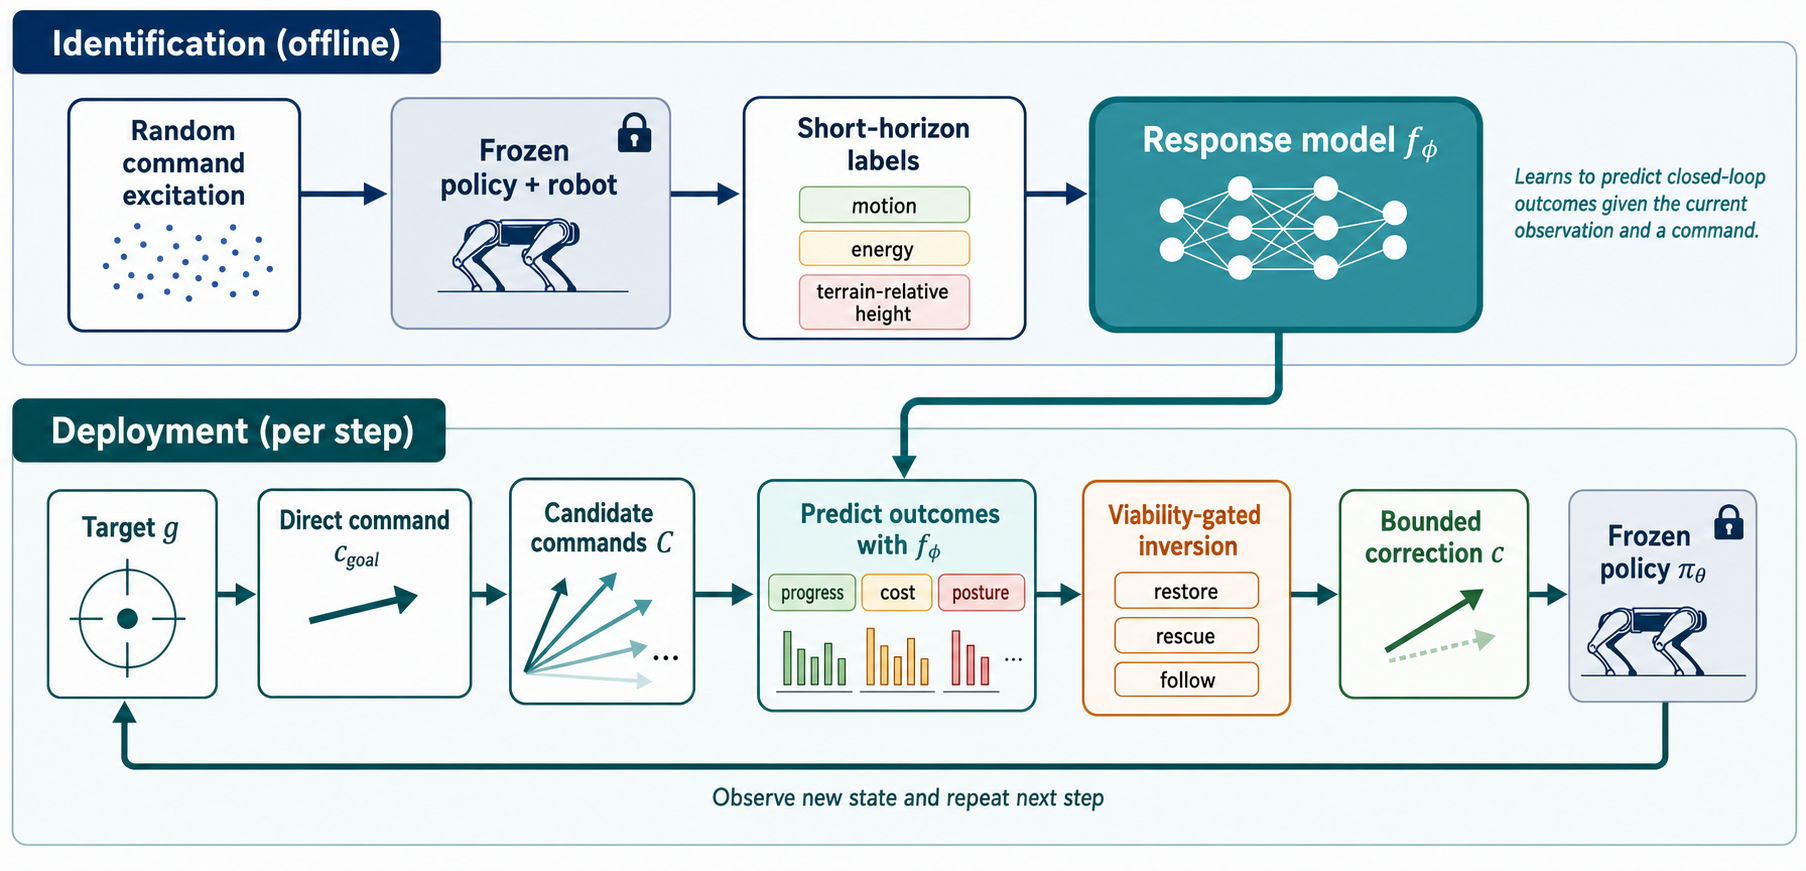
\includegraphics[width=\linewidth]{vgfc_method.png}
\caption{Overview of VGFC. \emph{Identification} (top, once and offline): the frozen policy is excited with random commands in closed loop with the robot, and a network $f_\phi$ regresses the short-horizon closed-loop response (body-frame motion, energy, and terrain-relative posture height) of each command. \emph{Deployment} (bottom, at each high-level step): the task target yields a proportional direct command $c_{\text{goal}}$; VGFC enumerates a candidate set around it, predicts each candidate's consequences with $f_\phi$, selects by viability-gated inversion the lowest-energy candidate that is progress-preserving and posture-safe, and applies the choice as a bounded correction $c$ that the frozen policy $\pi_\theta$ executes. The identified model conditions on the current observation, so the same command is scored differently across terrain and gait states.}
\label{fig:method}
\end{figure}

Figure~\ref{fig:method} summarizes the method.
VGFC has two phases: an offline \emph{identification} phase that fits a command-response model to the frozen policy's own excitation rollouts, and an online \emph{compensation} phase that, at each high-level step, enumerates candidate commands, predicts their consequences with that model, and applies a viability-gated, bounded correction to the task command before the frozen policy executes it.
The remainder of this section derives each component from a small set of design requirements.

\textbf{Design requirements.}
Three requirements shape every design decision that follows.
\emph{R1, no retraining}: the compensator must improve a policy whose weights, reward, and training pipeline are unavailable or too expensive to touch; it may only observe the policy acting.
\emph{R2, non-degradation}: the pretrained policy is already strong, so the compensator must be able to revert to it exactly, and every intervention must be rejected when its predicted benefit is uncertain.
\emph{R3, embodiment generality}: nothing in the method may depend on robot-specific knowledge beyond what can be identified automatically from the policy's own rollouts.
The resulting architecture has three parts, presented in the next three subsections: a compensation \emph{interface} (where to intervene, Section~\ref{sec:setting}), a response \emph{model} (what to know, Section~\ref{sec:model}), and a gated \emph{inversion} rule (how to act, Section~\ref{sec:vgfc}).

\subsection{Compensation Interface}
\label{sec:setting}

Let $\pi_\theta$ be a frozen, pretrained continuous-control policy mapping observations $o_t$ and a command $c$ to low-level actions.
In our locomotion instantiation $c = (v_x, v_y, \omega_z)$ is the body-frame velocity command, but the framework only requires \emph{some} command interface through which behavior can be steered, a property shared by learned controllers that are deployed as task-level building blocks~\citep{margolis2022walk,kumar2021rma}.

\textbf{Scope.}
Three properties of the policy, not of robots, delimit where the framework applies.
\emph{(i) A command interface must exist}: a single-task policy trained without conditioning exposes nothing to invert over, so VGFC does not apply to unconditioned RL policies (a limitation shared by every command-level method).
\emph{(ii) The interface must carry redundancy}: compensation exploits redundancy, that is, the existence of several commands that make comparable task progress at different cost; a task that fully determines the command admits no efficiency gain.
\emph{(iii) The closed loop must respond at a fast, roughly stationary timescale}: command consequences must be visible within a short prediction window, which holds when the policy stabilizes its plant (locomotion, end-effector servoing, vehicle velocity/curvature tracking) and fails for sparse, long-horizon credit-assignment problems.
These conditions characterize command-conditioned continuous control broadly, from legged robots to vehicle controllers, rather than reinforcement learning in general; Section~\ref{sec:limitations} returns to what lies outside them.

Why intervene at the command rather than at the action, as residual policy learning does~\citep{silver2018residual,johannink2019residual}?
Three reasons, mirroring the three requirements.
First, action-space corrections must be \emph{learned}, and learning them requires reward access and environment interaction, violating R1; a command-space correction can instead be \emph{computed} from an identified model.
Second, an action-space residual shares authority with the policy at the contact-critical timescale, where a wrong correction destabilizes; a command-space correction leaves $\pi_\theta$ in full control of posture, contacts, and joints, so the worst-case consequence of a poor command is inefficiency rather than loss of balance (R2).
Third, the command interface is the one interface that command-conditioned policies share across embodiments (R3): the same three command variables steer a quadruped and a humanoid.

A task supplies a target; throughout the method, $g$ denotes that target expressed in the robot's body frame at the current step, and the \emph{direct} controller computes a proportional command
\begin{equation}
c_{\text{goal}} \;=\; \bigl(\operatorname{clip}(k_v \, x_{\text{local}}), \; \operatorname{clip}(k_v \, y_{\text{local}}), \; \operatorname{clip}(k_\psi \operatorname{atan2}(y_{\text{local}}, x_{\text{local}}))\bigr),
\label{eq:cgoal}
\end{equation}
which is the uncompensated baseline: a strong pretrained policy driven straight at the goal.
Proportional commands of this kind are the standard way tasks are layered on velocity-conditioned policies, and they carry a systematic inefficiency: far from the goal they saturate, commanding full speed regardless of whether the terrain rewards it, and near the goal they shrink, producing energy-intensive in-place stepping.
Compensation replaces $c_{\text{goal}}$ with a corrected command at each high-level step (every $E = 4$ low-level steps).
The design question is where the correction comes from and when it is trusted.

\subsection{Command-Response Model}
\label{sec:model}

To correct a command before executing it, the compensator must predict what any candidate command would do.
The object to model is not the robot's action-level dynamics, as in model-based RL~\citep{nagabandi2018neural}: the policy already handles those competently, and re-modeling them would duplicate its work at far higher dimensionality.
The relevant object is the \emph{closed loop} of policy and robot, viewed from the command interface: for the current situation, it specifies the motion, energetic cost, and postural risk that each candidate command produces.
This reframing keeps the model input three-dimensional at the interface and makes identification a supervised problem on the policy's own rollouts, satisfying R1 and R3 simultaneously.

\textbf{Excitation data.}
We run the converged policy in $64$ parallel environments and override its command with excitation commands sampled uniformly from the command space (scaled down with probability $0.3$ to cover the near-goal regime), resampled every $25$ steps. This is system identification with persistent excitation, applied to the policy-robot closed loop.
Crucially, \emph{no quality filtering is applied}: stumbles, slips, and low-posture episodes are kept, because the model must know where the policy performs poorly.
This is the same self-distillation data source that populates our behavior archive (Section~\ref{sec:retrieval}); the difference is what is extracted from it.

\textbf{Response targets.}
The outputs instantiate a general three-channel schema that any instantiation of the framework must fill: a \emph{progress} statistic sufficient to score task advancement, the \emph{cost} being minimized, and the \emph{viability} quantity the gate guards.
For locomotion, from constant-command windows of $H{=}16$ low-level steps we regress six outcomes: body-frame displacement $(\Delta x, \Delta y)$ and yaw change $\Delta\psi$ (progress), per-step energy $\bar{e} = \operatorname{mean}(\lvert a_t \odot \dot{q}_t \rvert)$ (cost), and the minimum and mean of \emph{terrain-relative posture height} over the window (viability); a manipulation instantiation would substitute end-effector displacement, actuation effort, and a grasp-stability or joint-limit margin, and a vehicle instantiation path progress, consumption, and a slip margin.
The horizon is four replanning intervals ($E{=}4$ low-level steps per high-level decision, $80$\,ms at the $50$\,Hz control rate): long enough to span a stride and expose gait-level energy and posture differences between commands, short enough that a single-step prediction from the current observation remains accurate.
Posture height is recovered from the policy's own height-scan observation (mean scan return plus sensor offset), not from world coordinates.
This choice matters: on procedurally rough terrain, world-frame base height confounds posture with ground elevation, and a model trained on world-frame labels reaches only $R^2 = 0.25$ on minimum height; the terrain-relative labels raise this to $R^2 = 0.88$ (Table~\ref{tab:model}).
An unreliable height channel silently disables predictive gating; this label correction is what makes the viability gate work.

\textbf{Model.}
The response model is a mapping
\begin{equation}
f_\phi : (o_t, c) \;\longmapsto\; \bigl(\widehat{\Delta x}, \widehat{\Delta y}, \widehat{\Delta\psi}, \hat{e}, \hat{h}_{\min}, \hat{h}_{\text{mean}}\bigr),
\label{eq:responsemodel}
\end{equation}
where, here and throughout, hats mark quantities \emph{predicted} by the model and plain symbols are measured; $f_\phi$ is implemented as a two-layer MLP (256 units, dropout $0.1$) that takes the full policy observation with the command slice replaced by the candidate $c$; inputs and outputs are standardized, and training minimizes MSE with an episode-grouped train/test split so windows from one episode never straddle the split.
Conditioning on the full observation is what makes the predictions \emph{situational}: the same candidate command is predicted to cost different energy on different terrain and from different gait states, which is precisely the information a fixed command-shaping heuristic cannot express.
Identification is data-efficient: approximately 25k windows are obtained from roughly four minutes of parallel simulation, followed by a few minutes of training.

\subsection{Viability-Gated Inversion}
\label{sec:vgfc}

Given the response model, a naive compensator would select the command with the most favorable predicted outcome. Each safeguard introduced below addresses a distinct failure of this naive rule, quantified in Section~\ref{sec:ablation-vgfc}. Minimizing predicted distance-to-goal reduces the compensator to a speed maximizer, since aggressive commands are always favored over a short horizon; hence \emph{progress is treated as a constraint rather than the objective}. Minimizing energy without posture safeguards recovers the policy's true energetic optimum, a low-posture gait that fails the task; hence \emph{viability gates the objective}. Executing the optimizer's choice without attenuation concentrates all model error in the applied command; hence \emph{the correction is bounded}.

At each high-level step VGFC forms a candidate set $\mathcal{C}$ around the direct command: the direct command itself, scaled versions, yaw-rate perturbations, and a polar grid over approach speeds and angles with three yaw-rate levels ($\sim$70 candidates after deduplication).
A single batched forward pass predicts each candidate's response $(\widehat{\Delta x}, \widehat{\Delta y}, \widehat{\Delta\psi}, \hat{e}, \hat{h}_{\min}, \hat{h}_{\text{mean}})$, from which predicted progress is
\begin{equation}
\hat{P}(c) \;=\; \lVert g \rVert \;-\; \bigl\lVert g - (\widehat{\Delta x}(c), \widehat{\Delta y}(c)) \bigr\rVert .
\end{equation}
Selection then proceeds in one of three modes (Algorithm~\ref{alg:vgfc}):

\emph{(a) Follow (energy compensation).}
If the direct command is predicted posture-safe, VGFC selects
\begin{equation}
c^\ast \;=\; \arg\min_{c \,\in\, \mathcal{C}_{\text{elig}}} \; \hat{e}(c),
\qquad
\mathcal{C}_{\text{elig}} = \Bigl\{ c : \hat{P}(c) \ge \beta\, \hat{P}(c_{\text{goal}}), \;\;
\hat{h}_{\min}(c) \ge h_{\text{floor}}, \;\;
\hat{h}_{\text{mean}}(c) \ge h_{\text{now}} - \delta \Bigr\},
\label{eq:follow}
\end{equation}
with progress floor $\beta = 0.9$, posture floor $h_{\text{floor}}$ a fixed fraction of nominal posture height, and height-decline tolerance $\delta = 2$\,cm.
The compensation activates only if the predicted saving clears a relative margin, $\hat{e}(c^\ast) < (1 - \epsilon)\, \hat{e}(c_{\text{goal}})$ with $\epsilon = 0.1$; otherwise the direct command runs unmodified.
The semantics are exactly feedforward compensation: \emph{keep the reference trajectory, remove the systematic energetic inefficiency}.

\emph{(b) Rescue (predictive viability).}
If the \emph{direct command itself} is predicted to drive minimum posture height below a rescue threshold $h_{\text{resc}}$ (set below the eligibility floor $h_{\text{floor}}$, so ordinary roughness does not trigger it), meaning the model foresees height collapse, VGFC instead selects the candidate maximizing predicted minimum posture height among those with non-negative predicted progress.
This is the gate acting before failure exists: reactive height gates triggered by \emph{measured} height, which we tested in the retrieval variant, either block progress or fire after posture is already lost.

\emph{(c) Restore (measured posture).}
If measured posture height has already sagged below an operating band, compensation is suspended and the direct command runs until posture recovers; the aggressive proportional command restores height reliably.
This closes the loop against slow posture drift that a 16-step model horizon cannot see.

\textbf{Bounded, annealed correction.}
In all modes the selected candidate is applied as a \emph{bounded feedforward correction} rather than a substitute, and the correction gain decays as the goal approaches:
\begin{equation}
c \;=\; c_{\text{goal}} + \alpha \,\bigl(c^\ast - c_{\text{goal}}\bigr),
\qquad
\alpha \;=\; \alpha_0 \operatorname{clip}\!\bigl(\nicefrac{\lVert g \rVert}{d_{\text{anneal}}},\, 0,\, 1\bigr),
\qquad \alpha_0 = 0.5 .
\label{eq:blendff}
\end{equation}
Bounding ($\alpha_0 < 1$) means the compensator biases the reference toward the model's preferred command but never fully owns it; this is the classical feedforward posture (correct the reference, keep the controller), and Section~\ref{sec:ablation-vgfc} shows it is what makes the method robust to model error: full substitution matches the bounded correction on the tuning seed and loses 5--6 success points off it.
Annealing ($d_{\text{anneal}} = 0.5$\,m) returns full authority to the base policy for the terminal approach, because the success criterion is evaluated at the terminal state, which lies beyond the model's prediction horizon for most of the episode.
The three modes are checked in the order restore, rescue, follow, so measured evidence overrides predicted evidence.
The runtime cost of the compensator is negligible: a single batched forward pass over all candidates requires $0.14$\,ms on CPU ($0.08$\,ms on GPU), against the $80$\,ms high-level control interval.

Altogether VGFC exposes seven scalars: the progress floor $\beta = 0.9$, the posture floors $h_{\text{floor}}$ and $h_{\text{resc}}$ ($0.85$ and $0.80$ of nominal height), the restore band ($0.90$), the relative energy margin $\epsilon = 0.1$, and the correction gain $\alpha_0$ and annealing distance $d_{\text{anneal}}$ of Eq.~\ref{eq:blendff}.
All were tuned once, on a single seed of one robot, and frozen for every robot and task family we evaluate (Section~\ref{sec:setup}).

\begin{algorithm}[t]
\caption{Viability-Gated Feedforward Compensation (one high-level step)}
\label{alg:vgfc}
\begin{algorithmic}[1]
\Require frozen policy $\pi_\theta$, response model $f_\phi$, target $g$, scalars $(\beta, h_{\text{floor}}, h_{\text{resc}}, \delta, \epsilon, \alpha_0, d_{\text{anneal}})$
\State Compute body-frame target $g$ and direct command $c_{\text{goal}}$ (Eq.~\ref{eq:cgoal})
\State Build candidate set $\mathcal{C}$; predict responses $f_\phi(o, c)$ for all $c \in \mathcal{C}$ in one batch
\If{measured posture $h_{\text{now}} <$ operating band}  \Comment{restore}
  \State $c^\ast \gets c_{\text{goal}}$
\ElsIf{$\hat{h}_{\min}(c_{\text{goal}}) < h_{\text{resc}}$}  \Comment{rescue: predicted collapse}
  \State $c^\ast \gets \arg\max_{c\,:\,\hat{P}(c) \ge 0} \hat{h}_{\min}(c)$
\Else  \Comment{follow: energy compensation}
  \State $c^\ast \gets \arg\min_{c \in \mathcal{C}_{\text{elig}}} \hat{e}(c)$ per Eq.~\ref{eq:follow}
  \If{$\hat{e}(c^\ast) \ge (1 - \epsilon)\, \hat{e}(c_{\text{goal}})$} $c^\ast \gets c_{\text{goal}}$ \EndIf
\EndIf
\State Execute $\pi_\theta$ with $c = c_{\text{goal}} + \alpha (c^\ast - c_{\text{goal}})$ for $E$ low-level steps \Comment{bounded, annealed; Eq.~\ref{eq:blendff}}
\end{algorithmic}
\end{algorithm}

\subsection{Retrieval Variant (VGSR)}
\label{sec:retrieval}

Before arriving at model inversion, we developed \emph{Viability-Gated Skill Residuals} (VGSR), which we report in full as the natural skill-archive alternative.
The same converged-policy rollouts are segmented into chunks, described by body-frame outcome descriptors (displacement, velocities, yaw rate, height statistics, energy, stability, smoothness), filtered by utility and descriptor novelty, and clustered into an online quality-diversity-style archive~\citep{cully2015robots}.
At deployment, a chunk is selected by a descriptor-level cost combining predicted progress, initial-state applicability, energy, stability, and utility; its velocity descriptor is converted into a command that is \emph{blended} with the direct command, $c = (1-\lambda)\, c_{\text{goal}} + \lambda\, c_{\text{skill}}$, with $\lambda > 0$ only when a heuristic viability gate (goal alignment, predicted progress, chunk stability, energy z-score, speed cap) accepts the candidate; a learned decision-level gate can further filter it.
VGSR is the non-parametric counterpart of VGFC: retrieval interpolates only where the archive has coverage, while the response model interpolates over the entire command space; and VGSR's gate checks properties \emph{of an archived chunk}, while VGFC's gate checks \emph{predicted consequences of the actual candidate command in the current state}.
Section~\ref{sec:results-retrieval} quantifies the difference.

\section{Experiments}
\label{sec:results}

Our experiments answer four questions.
\emph{Q1}: does compensation improve a strong pretrained policy, and on which metrics (Sections~\ref{sec:results-harder},~\ref{sec:results-coverage})?
\emph{Q2}: does the recipe transfer across embodiments without re-tuning (Section~\ref{sec:results-coverage})?
\emph{Q3}: which components carry the effect (Section~\ref{sec:ablation-vgfc})?
\emph{Q4}: how does model inversion compare with the retrieval-based use of the same experience (Section~\ref{sec:results-retrieval})?

\subsection{Setup}
\label{sec:setup}

\textbf{Environments and robots.}
All experiments use Isaac Lab~\citep{mittal2023orbit} rough-terrain velocity environments with three embodiments: \texttt{Isaac-Velocity-Rough-Unitree-Go2-v0} and \texttt{Isaac-Velocity-Rough-Anymal-D-v0} (quadrupeds) and \texttt{Isaac-Velocity-Rough-H1-v0} (humanoid), with the publicly distributed pretrained RSL-RL checkpoints~\citep{rudin2022learning,schwarke2025rslrl} as the compensated policies.
The task is target reaching: move the base to a target $g$ specified relative to the start pose.
Success requires no early termination, final XY distance below $0.3$\,m, and \emph{final height} above $70\%$ of spawn height.
Final height is the world-frame height of the base at the episode's last step; it serves as a terminal posture check, so that an episode that reaches the target crouched, collapsed, or mid-fall does not count as a success.
Because the terrain is procedurally rough, final height reflects both posture and the ground elevation at wherever the robot stops, which is why we report it alongside, rather than inside, the energy and distance metrics.
We also report final distance, the energy proxy $\operatorname{mean}(\lvert a \odot \dot{q}\rvert)$ (mean absolute mechanical power over the episode), and how often compensation was active.

\textbf{Task families.}
\emph{Harder} Go2 targets: $(2,0)$, $(1.5,1)$, $(0,1.25)$, $(-0.75,0)$, $(1,-1)$, $(0,-1.25)$, $(-1,0.75)$, $(1.75,-0.75)$\,m: long, diagonal, lateral, and backward goals covering the command space (the last three directions were added when the benchmark was expanded and were never used in any tuning).
\emph{Moderate} Go2 targets: $(0.75,0)$, $(0.75,0.75)$, $(1.5,0)$, $(0,0.75)$\,m.
\emph{Holdout} Go2 directions (never used during any tuning): $(1.25,0.5)$, $(0.5,1)$, $(-0.5,0.5)$, $(1.25,-0.5)$\,m.
ANYmal-D and H1 use the same eight harder targets as Go2. Excitation collection, identification, and every gate parameter are shared unchanged across the two quadrupeds (Go2 and ANYmal-D). The humanoid reuses this configuration in full except for the posture floor, which is set more conservatively to reflect its higher center of mass and smaller support region (Section~\ref{sec:results-coverage}); in particular the energy margin, the objective, and the response-model architecture are identical across all three robots. The only per-robot components are thus the identified response model and, for the morphologically distinct humanoid, the posture floor, both determined by physical properties rather than tuned to the benchmark.

\textbf{Methods.}
(1)~\texttt{direct}: the pretrained policy under the direct target command (the policy being compensated, and a strong baseline);
(2)~\texttt{VGSR}: the retrieval-based variant with heuristic gate (and recovery clause on harder targets);
(3)~\texttt{VGFC}: model-feedforward compensation (Section~\ref{sec:vgfc}).
Random/zero-command baselines are excluded as uninformative against a strong pretrained policy.

\textbf{Protocol.}
VGFC's seven scalars (Section~\ref{sec:vgfc}) were tuned on a \emph{single} seed (301) on the harder set only, then frozen.
All reported results use disjoint evaluation seeds: harder $5$ seeds $\times$ $10$ trials $\times$ $8$ targets (400 episodes per method), moderate $3 \times 10$ (120), holdout $3 \times 5$ (60), ANYmal-D $3 \times 5 \times 8$ (120), H1 $3 \times 5 \times 8$ (120).
Per-robot response models (Go2, ANYmal-D, H1) are identified with the identical recipe.
We report episode-level bootstrap 95\% CIs.

\subsection{Response-Model Quality}
\label{sec:results-model}

Table~\ref{tab:model} reports held-out-episode test metrics for the Go2 response model.
Displacement and yaw responses are accurately predicted ($R^2 \ge 0.92$); energy is predicted well enough to rank candidates ($R^2 = 0.75$); and terrain-relative posture height is predicted reliably ($R^2 = 0.88$/$0.91$ for min/mean, MAE under $9$\,mm), versus $R^2 = 0.25$ when the same model is trained on world-frame height labels, which terrain elevation corrupts.
The excitation data also matters: an earlier model trained on utility-filtered archive segments (the natural ``reuse the archive'' shortcut) reached $R^2 = -1.9$ on lateral displacement, because curated high-quality segments underrepresent exactly the sloppy behavior the model must know about.

\textbf{Identification data efficiency.}
Re-identifying the model from episode-group subsamples of the excitation data degrades gracefully: with $50\%$ of the data, displacement $R^2$ holds at $0.93$ and energy drops to $0.72$; with $25\%$ ($\approx$ one minute of parallel simulation), displacement is still $0.92$ and energy $0.62$.
Displacement, which drives the progress constraint, saturates early; accuracy on energy, the quantity being optimized, is what additional data improves.
Section~\ref{sec:ablation-vgfc} evaluates the $25\%$ model in closed loop.

\begin{table}[t]
\centering
\caption{Go2 command-response model, held-out-episode test metrics ($\sim$25k excitation windows, 16-step horizon). Terrain-relative height labels are essential for the viability gate.}
\label{tab:model}
\begin{tabular}{lccc}
\toprule
Output & MAE & RMSE & $R^2$ \\
\midrule
$\Delta x$ (m)            & 0.019 & 0.025 & 0.944 \\
$\Delta y$ (m)            & 0.019 & 0.025 & 0.942 \\
$\Delta \psi$ (rad)       & 0.029 & 0.042 & 0.927 \\
energy (per step)         & 0.435 & 0.625 & 0.752 \\
min.\ rel.\ height (m)    & 0.009 & 0.012 & 0.875 \\
mean rel.\ height (m)     & 0.008 & 0.010 & 0.906 \\
\midrule
min.\ height, world-frame labels & 0.039 & 0.092 & 0.247 \\
\bottomrule
\end{tabular}
\end{table}

\subsection{Go2 Harder Targets: Main Result}
\label{sec:results-harder}

The harder-target benchmark comprises eight targets (five original plus three added directions, Section~\ref{sec:setup}) evaluated over 5 seeds $\times$ 10 trials, i.e.\ 400 episodes per method.

\textbf{Aggregate.}
VGFC reduces energy by $10.5\%$ ($1.976$ vs.\ $2.208$; CIs $[1.938, 2.016]$ vs.\ $[2.156, 2.256]$, non-overlapping) while success is statistically matched ($0.797$, CI $[0.760, 0.835]$, vs.\ $0.805$, CI $[0.765, 0.843]$), with matched final distance and height and zero early terminations for either method.
The energy effect is consistent \emph{within} seeds: the paired per-seed difference is negative on all five benchmark seeds ($-6.4\%$ to $-14.3\%$), and on all 17 evaluation seeds across the Go2 families, ANYmal-D, and H1 (sign test $p < 10^{-5}$), while the paired success difference is centered on zero ($-0.05$ to $+0.04$).
Figure~\ref{fig:paired} visualizes both distributions. We report the aggregate in text rather than as a bar chart, since the finding reduces to a single energy reduction alongside a null effect on success, which a grouped bar chart would not convey more clearly.
The retrieval variant, evaluated on the original five-target protocol (250 episodes), reaches a similar per-family energy level ($2.061$ vs.\ VGFC's $2.073$ under that protocol) but with a $1.2\%$ termination rate and lower final height, and, as Section~\ref{sec:results-retrieval} shows, its savings do not persist across the other task families.

\begin{figure}[t]
\centering
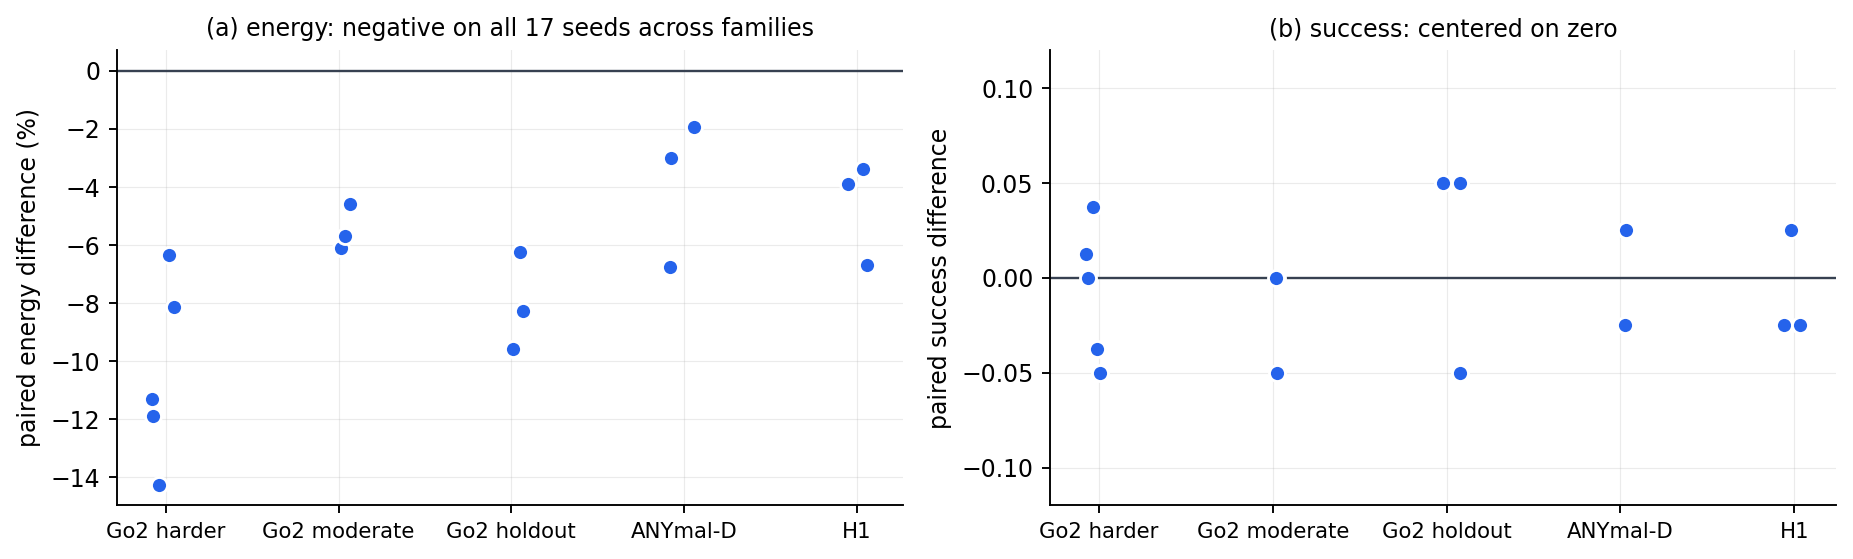
\includegraphics[width=0.85\linewidth]{ff_v4_paired_differences.png}
\caption{Paired per-seed differences (VGFC $-$ direct, evaluated inside the same runs) for every evaluation seed of every task family. Left: the relative energy difference is negative on all 17 evaluation seeds across the five task-family/embodiment combinations (sign test $p < 10^{-5}$). Right: the success difference is centered on zero. Compensation reduces energy without a corresponding reduction in success.}
\label{fig:paired}
\end{figure}

\begin{figure}[t]
\centering
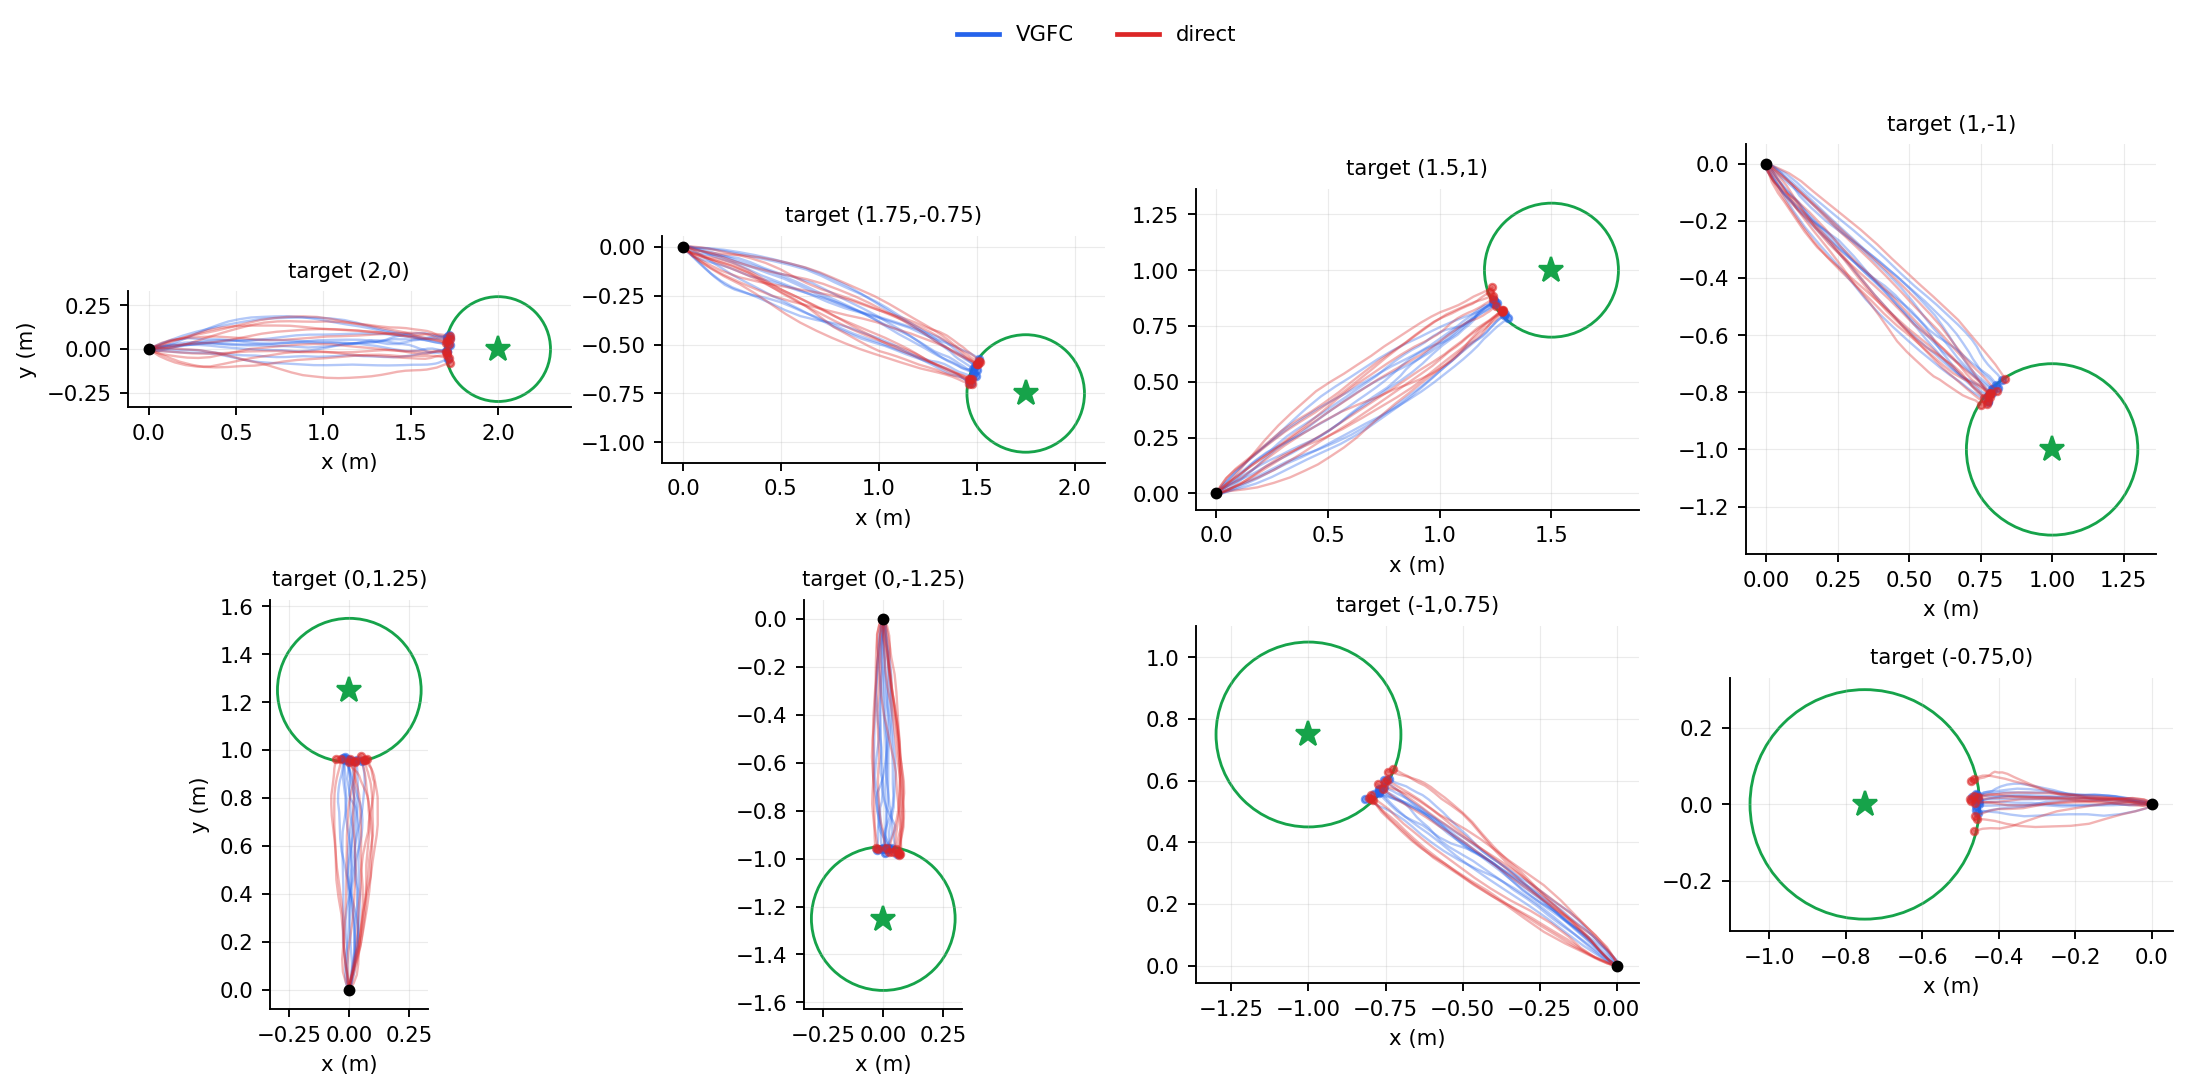
\includegraphics[width=\linewidth]{ff_v4_harder_trajectories.png}
\caption{Control examples: XY paths on the eight harder targets (one evaluation seed, 10 trials per method; the green circle is the success radius). VGFC and the direct baseline reach the same target neighborhoods along closely matched paths; the compensation changes how the command is tracked, not where the robot goes.}
\label{fig:traj}
\end{figure}

\begin{figure}[t]
\centering
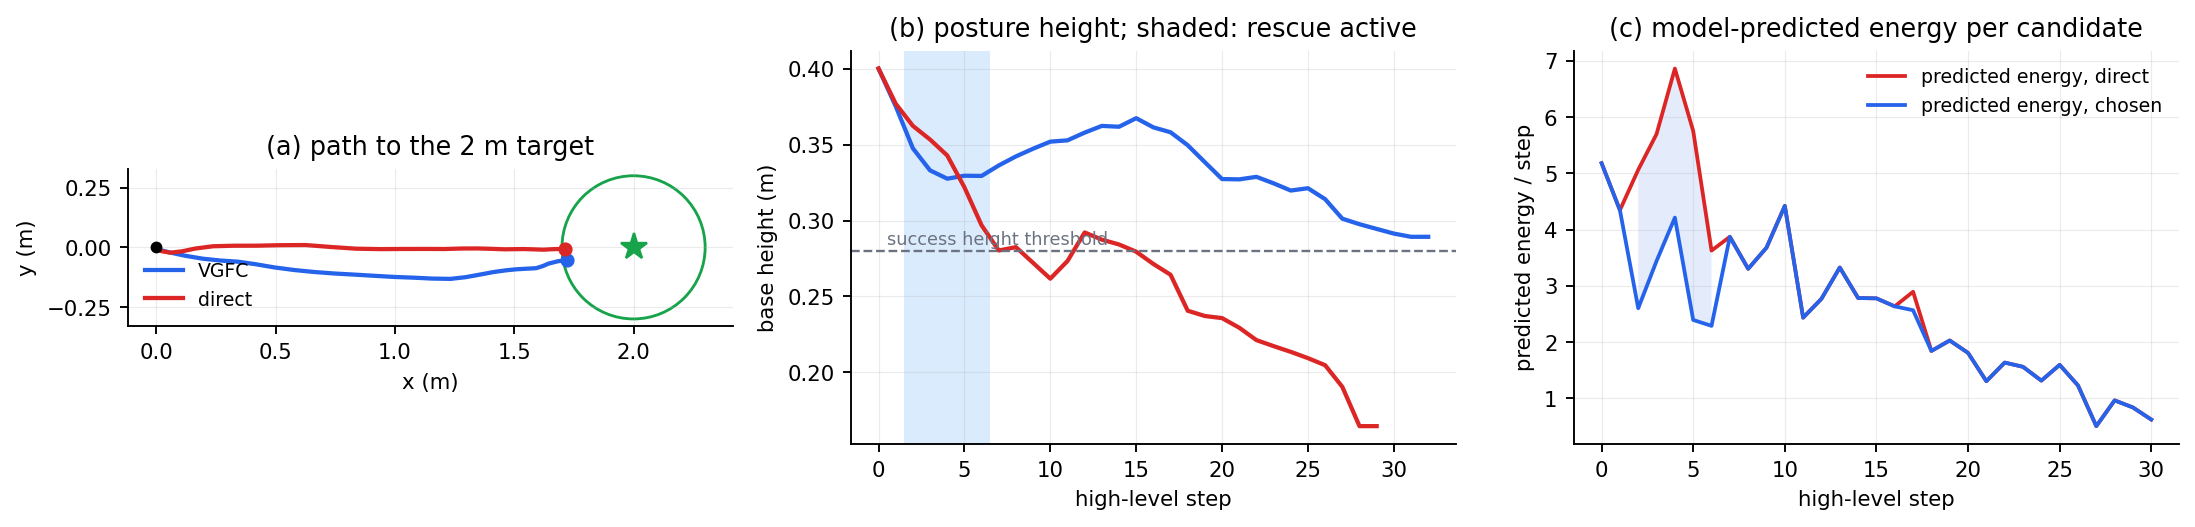
\includegraphics[width=\linewidth]{ff_v4_control_example.png}
\caption{A single compensated episode on the hardest target $(2,0)$. (a)~Both controllers walk 2\,m over rough terrain. (b)~Base height over the episode: during the shaded steps the model predicts that the direct command would breach the posture floor, and the rescue mode substitutes height-preserving candidates; VGFC maintains posture while the uncompensated policy falls below the success threshold. (c)~The response model's per-step energy predictions for the direct command and the chosen candidate; the shaded gap is the predicted saving that the margin requires before compensating.}
\label{fig:example}
\end{figure}

\textbf{Control examples.}
Figure~\ref{fig:traj} overlays the closed-loop XY paths for all trials of one evaluation seed: compensated and uncompensated trajectories are nearly indistinguishable in space, which is the intent, since the compensation acts on command tracking rather than on the route.
Figure~\ref{fig:example} dissects a single episode on the hardest target and shows the predictive rescue mechanism at work: the model forecasts a posture-floor breach early in the walk, rescue-mode candidates maintain the base height through the critical segment, and the episode terminates at nominal posture, whereas the direct baseline falls below the success threshold.

\textbf{Per-target (Table~\ref{tab:pertarget}).}
The per-target breakdown accounts for the aggregate result.
Energy improves on seven of eight targets (up to $-14\%$), with the one exception, the short backward goal, at parity; final height is within a few millimeters everywhere.
Success differences vary in both directions at the per-target sample size ($n{=}50$): the long diagonal $(1.5,1)$ favors VGFC ($0.800$ vs.\ $0.740$, the target the annealed correction is designed to protect), the two long forward and diagonal goals favor the direct baseline by a comparable margin, and the remaining five are matched.
We make no claim of a single-target success effect: across protocol versions these $n{=}50$ differences varied by $\pm 0.1$ while the energy ordering remained unchanged, a pattern consistent with a genuine energy effect and a null effect on success.

\textbf{On final height.}
Compensated final height is $1$--$3$\,mm below the baseline on the Go2 families ($0.3228$ vs.\ $0.3253$ here, with near-identical CIs).
This effect is inherent to the objective: among posture-safe candidates the energy minimizer favors marginally gentler commands, and on a velocity-conditioned policy gait vigor and carried height are weakly coupled, so the lowest-energy safe gait is marginally lower in height.
The posture floors and the restore mode bound this coupling to the millimeter scale (early unconstrained variants lost centimeters, and the task, with them; Section~\ref{sec:ablation-vgfc}); on ANYmal-D final height is identical to the baseline, and on H1 it is within $1.3$\,cm, the conservative posture floor keeping the compensated humanoid close to the base policy's carriage (Table~\ref{tab:coverage}).

\textbf{On the residual failure mode.}
Every failure on this benchmark, for both methods (81 and 78 of 400 episodes respectively), is of a single kind: the robot reaches the target region but finishes below the height criterion after its gait has settled low over the walk.
We examined whether a posture-aware stopping rule could recover these episodes: under a symmetric protocol in which \emph{neither} controller may terminate the task while posture is low (the direct baseline continues tracking; VGFC selects the candidate with the highest predicted posture among those remaining within the target region), success does not improve for either method at $n{=}400$ per method; episodes instead expend their remaining budget attempting recovery, occasionally falling (early terminations appear for both methods), and the additional low-motion steps inflate the denominator of the per-step energy metric.
Individual episodes are recoverable, as Figure~\ref{fig:example} illustrates, but in aggregate the low-posture arrival state is governed by terrain and gait-settling dynamics that command-level intervention does not reliably reverse.
This delimits what any compensator operating at this interface can achieve on this success criterion, and is why our principal claim concerns energy at matched success rather than success itself.

\begin{table}[t]
\centering
\caption{Per-target breakdown on the eight harder targets (50 episodes per target per method), ordered by the paired energy saving. Energy improves on seven of eight targets, by up to $12.9\%$; success differences at this sample size scatter in both directions around parity, and final height is matched to a few millimeters.}
\label{tab:pertarget}
\begin{tabular}{lccccccc}
\toprule
& \multicolumn{3}{c}{Energy $\downarrow$} & \multicolumn{2}{c}{Success $\uparrow$} & \multicolumn{2}{c}{Final height (m)} \\
\cmidrule(lr){2-4}\cmidrule(lr){5-6}\cmidrule(lr){7-8}
Target (m) & VGFC & direct & $\Delta$ & VGFC & direct & VGFC & direct \\
\midrule
$(0,1.25)$           & \textbf{1.815} & 2.083 & $\mathbf{-12.9\%}$ & 0.940 & 0.980 & 0.340 & 0.351 \\
$(1.75,-0.75)$       & \textbf{2.217} & 2.542 & $\mathbf{-12.8\%}$ & 0.480 & 0.520 & 0.276 & 0.285 \\
$(-1,0.75)$          & \textbf{1.861} & 2.122 & $\mathbf{-12.3\%}$ & 1.000 & 1.000 & 0.358 & 0.367 \\
$(0,-1.25)$          & \textbf{1.822} & 2.073 & $\mathbf{-12.1\%}$ & 0.940 & 0.980 & 0.345 & 0.350 \\
$(1.5,1)$            & \textbf{2.203} & 2.471 & $\mathbf{-10.8\%}$ & 0.800 & 0.740 & 0.316 & 0.313 \\
$(2,0)$              & \textbf{2.367} & 2.619 & $\mathbf{-9.6\%}$  & 0.240 & 0.260 & 0.233 & 0.224 \\
$(1,-1)$             & \textbf{2.028} & 2.240 & $\mathbf{-9.5\%}$  & 0.980 & 0.960 & 0.355 & 0.349 \\
$(-0.75,0)$          & 1.496 & \textbf{1.510} & $-0.9\%$ & 1.000 & 1.000 & 0.359 & 0.363 \\
\bottomrule
\end{tabular}
\end{table}

\subsection{Systematic Coverage: Moderate, Holdout, and H1}
\label{sec:results-coverage}

A compensation layer must improve performance where the base policy is weak, avoid degrading it where the base policy is strong, and transfer across embodiments without manual tuning.
Table~\ref{tab:coverage} evaluates the configuration on the remaining Go2 target families and on two further robots, ANYmal-D and H1, using the same eight-target benchmark for the cross-embodiment rows.

\begin{table}[t]
\centering
\caption{Systematic coverage on the eight-target benchmark (moderate and holdout are additional Go2-specific target sets). Energy $\Delta$ is VGFC relative to the direct baseline evaluated inside the same runs. Success is statistically matched in every family and energy is reduced in every family; the paired per-seed energy difference is negative on all evaluation seeds (Go2 and ANYmal-D under the shared quadruped configuration; H1 with the posture floor matched to the humanoid, Section~\ref{sec:setup}).}
\label{tab:coverage}
\begin{tabular}{llcccc}
\toprule
Family ($n$/method) & Method & Success $\uparrow$ & Energy $\downarrow$ & Energy $\Delta$ & Final height (m) \\
\midrule
\multirow{2}{*}{Go2 moderate (120)}
 & VGFC   & 0.975 {\scriptsize$[0.942, 1.000]$} & \textbf{1.743} {\scriptsize$[1.689, 1.802]$} & $-5.4\%$ & 0.356 \\
 & direct & \textbf{0.992} {\scriptsize$[0.975, 1.000]$} & 1.844 {\scriptsize$[1.763, 1.932]$} & -- & \textbf{0.362} \\
\midrule
\multirow{2}{*}{Go2 holdout (60)}
 & VGFC   & \textbf{0.933} {\scriptsize$[0.867, 0.983]$} & \textbf{1.936} {\scriptsize$[1.836, 2.037]$} & $-8.0\%$ & \textbf{0.334} \\
 & direct & 0.917 {\scriptsize$[0.833, 0.983]$} & 2.105 {\scriptsize$[1.982, 2.234]$} & -- & 0.333 \\
\midrule
\multirow{2}{*}{ANYmal-D, 8 targets (120)}
 & VGFC   & \textbf{0.883} {\scriptsize$[0.825, 0.942]$} & \textbf{1.367} {\scriptsize$[1.317, 1.422]$} & $-3.9\%$ & 0.500 \\
 & direct & 0.875 {\scriptsize$[0.817, 0.933]$} & 1.422 {\scriptsize$[1.373, 1.471]$} & -- & 0.500 \\
\midrule
\multirow{2}{*}{H1, 8 targets (120)}
 & VGFC   & 0.967 {\scriptsize$[0.933, 0.992]$} & \textbf{0.690} {\scriptsize$[0.665, 0.716]$} & $-4.7\%$ & 0.928 \\
 & direct & \textbf{0.975} {\scriptsize$[0.942, 1.000]$} & 0.724 {\scriptsize$[0.696, 0.752]$} & -- & \textbf{0.941} \\
\bottomrule
\end{tabular}
\end{table}

\textbf{Moderate and holdout targets.}
Energy drops on both families ($-5.4\%$ and $-8.0\%$) at statistically matched success ($0.975$ vs.\ $0.992$ and $0.933$ vs.\ $0.917$, CIs overlapping in both directions).
The holdout family is the most informative case: these directions were not observed during any tuning, so the frozen gates generalize across the command space, a property the retrieval variant does not possess (Section~\ref{sec:results-retrieval}: the archive variant \emph{increases} energy on these directions).

\textbf{Third embodiment, zero re-tuning: ANYmal-D.}
Applying the recipe unchanged to a different quadruped on the full eight-target benchmark reduces energy by $3.9\%$ at matched success ($0.883$ vs.\ $0.875$), with identical final posture and zero terminations; the paired energy difference is negative on all three ANYmal seeds.
Since not a single parameter was adjusted, this indicates that the compensation exploits a structural property of proportional command tracking on rough terrain rather than an artifact specific to the Go2 policy, and that the identification recipe is the only per-robot component the method needs.
(The retrieval variant is absent from this row by construction: VGSR requires building and curating a per-robot behavior archive, which is exactly the dependency the response model removes.)

\textbf{H1 humanoid: the safeguard is posture, not the energy margin.}
On the same eight-target benchmark, VGFC reduces H1 energy by $4.7\%$ at matched success ($0.967$ vs.\ $0.975$), with the paired energy difference negative on all three seeds ($-3.4\%$, $-3.9\%$, $-6.7\%$) and per-target savings up to $11\%$.
Reaching this required identifying the humanoid's distinct failure mode.
With the quadruped gate applied unchanged, an aggressive energy margin does capture savings but drives the tall, high-inertia H1 into posture collapse on the long forward and diagonal targets, costing success (the $2$\,m target falls to $0.47$ success): the failure is loss of balance, not an energy misprediction.
The remedy is morphological rather than a re-tuning of the objective: a humanoid has a substantially higher center of mass and a smaller support region than a quadruped, so its posture floors must be more conservative.
With the posture floor tightened accordingly (the single gate parameter that reflects morphology) and every other parameter, including the energy margin, left identical to the quadruped configuration, the gate admits only posture-safe candidates, and the energy savings are recovered at matched success.
H1 therefore extends the result to a third, morphologically distinct embodiment, and localizes the one quantity that a new morphology class requires: the posture safeguard, set from the robot's stability geometry rather than tuned to the benchmark.

\subsection{Retrieval-Based Compensation}
\label{sec:results-retrieval}

The retrieval variant was evaluated extensively before VGFC existed; we first compare head-to-head, then summarize the study it produced.

\textbf{Head-to-head.}
The three methods were evaluated inside the same runs on the original five-target protocol (5 seeds $\times$ 10 trials, 250 episodes per method, pre-annealing VGFC configuration).
There, VGSR reaches VGFC's energy level on the harder family ($2.061$ vs.\ $2.073$, both $\approx 12\%$ below direct) but with a $1.2\%$ termination rate and lower final height; on moderate targets its saving is smaller at lower success; and on holdout directions and H1 it \emph{increases} energy ($+3.8\%$, $+4.4\%$), where VGFC reduces energy ($-8\%$) or remains neutral.
The pattern reflects the coverage argument of Section~\ref{sec:retrieval}: retrieval performs well where the archive is dense (the harder targets around which it was constructed) and degrades outside that support, whereas the response model generalizes across the command space.

\textbf{Multi-seed aggregate.}
In a five-seed, 200-episode-per-method aggregate on the harder targets, VGSR reduced energy by $7.8\%$ ($1.99$ vs.\ $2.16$, non-overlapping bootstrap CIs) at statistically indistinguishable success ($0.785$ vs.\ $0.800$): consistent, but smaller than VGFC's gains and without success improvement.

\textbf{Gate necessity.}
Removing VGSR's gate leaves final distance intact but inflates energy by over $50\%$ ($3.18$ vs.\ $2.08$), with the residual activating at nearly twice the gated rate: without an activation mechanism, the archive yields a net increase in energy.

\textbf{Archive capacity is not the determining factor.}
Trimming the 3{,}904-chunk archive to its top-2{,}000 chunks by utility \emph{improved} success on a shared seed ($0.840$ vs.\ $0.680$), while a top-500 archive gave the lowest energy ($1.75$) at reduced success ($0.760$); all sizes reduced energy versus direct.
Quality filtering, rather than capacity, is what makes the retrieval variant effective, and its non-monotonic dependence on archive size is a tuning burden that the response model avoids.

\textbf{Learned decision gates.}
A decision-level viability classifier trained on logged gate decisions (episode-group split, heuristic-gate outputs excluded from inputs) reaches AUC $0.97$, and deployed in intersection with the physical guard it is stable on held-out directions; but trained on episode-level success labels it learns ``low-energy, goal-approaching'' as a proxy and loses success on the height-limited 2\,m target.
VGFC's gate resolves exactly this: its safety signal is a \emph{predicted physical quantity} (posture height) rather than a correlate of episode outcome.

\subsection{Ablating VGFC's Components}
\label{sec:ablation-vgfc}

Which parts of VGFC carry the result?
We ablate one component at a time on the eight-target benchmark under a shared protocol (2 seeds $\times$ 5 trials $\times$ 8 targets $=$ 80 episodes per variant), reporting each variant's paired difference against the direct baseline evaluated in the same runs (Table~\ref{tab:vgfc-ablation}):
\emph{no annealing} disables the goal-proximity decay of the correction gain;
\emph{no gate} removes all posture safeguards (height floors, rescue, and restore), leaving only the progress floor;
\emph{no progress floor} sets $\beta = 0$, leaving only the posture safeguards;
\emph{substitution} sets $\alpha = 1$, executing the selected candidate verbatim;
and \emph{25\% data} uses a response model identified from a quarter of the excitation data ($\approx$ one minute of simulation).

\begin{table}[t]
\centering
\caption{VGFC component ablations on the eight-target benchmark (2 seeds $\times$ 5 trials $\times$ 8 targets $=$ 80 episodes per variant). Each row removes or alters one component. All quantities are \emph{paired} differences against the direct baseline evaluated in the same runs, which controls for the seed subset and is the only measure comparable across variants; absolute values at this scale are not the calibrated numbers (Section~\ref{sec:results-harder}), and at $n{=}80$ paired success differences below $\sim$0.08 are at the noise level. ``Active steps'' is the mean number of high-level steps per episode (of a $\sim$40-step budget) at which compensation is applied.}
\label{tab:vgfc-ablation}
\begin{tabular}{lccc}
\toprule
Variant & $\Delta$ energy $\downarrow$ & $\Delta$ success & Active steps \\
\midrule
VGFC (full)                 & $-12.2\%$ & $+0.012$ & 11.7 \\
\midrule
no annealing                & $-12.2\%$ & $+0.013$ & 12.3 \\
no viability gate           & $-4.8\%$  & $-0.025$ & 8.9 \\
no progress floor           & $-19.6\%$ & $-0.037$ & 19.8 \\
substitution ($\alpha{=}1$) & $-14.0\%$ & $-0.050$ & 16.3 \\
25\% identification data    & $-6.4\%$  & $-0.012$ & 10.7 \\
\bottomrule
\end{tabular}
\end{table}

The ablations separate the components' roles.
\textbf{The gate converts predicted savings into realized ones.}
Removing the posture safeguards does not unleash deeper savings; it forfeits most of them ($-4.8\%$ vs.\ $-12.2\%$) while flipping the paired success difference negative: candidates that look efficient to the model but leave the well-behaved posture regime burn their predicted savings in the recovery dynamics that follow.
The viability gate is not a tax on compensation; it is the mechanism by which open-loop predictions survive contact with the closed loop.
\textbf{The progress floor bounds behavioral drift.}
Without it the compensator is active at nearly every step (19.8 vs.\ 11.7) and realizes the deepest raw saving ($-19.6\%$), but the paired success difference is the second worst in the table and posture is lower; the floor is the conservative tether that keeps the compensated trajectory recognizable as the commanded task.
\textbf{Bounding the correction is the robustness mechanism.}
Substitution pays the largest paired success cost ($-5.0$ points here, $-6.4$ points in an earlier 250-episode five-seed protocol) for savings the bounded correction largely retains.
\textbf{Annealing acts as posture insurance rather than an energy-reduction mechanism.}
Disabling the goal-proximity decay leaves aggregate energy unchanged ($-12.2\%$ either way); the component exists to return terminal-approach authority to the base policy, and its effect is target-specific rather than aggregate.
\textbf{Identification is data-efficient and degrades gracefully.}
With a quarter of the excitation data ($\approx$ one minute of simulation), success stays at parity and the saving shrinks from $-12.2\%$ to $-6.4\%$: the binding resource is the energy channel's accuracy ($R^2$ $0.62$ vs.\ $0.75$), precisely the channel the margin guards, and the safety components hold regardless.

Two further design choices are supported by earlier evidence at scale.
\textbf{Full substitution degrades off the tuning seed}: across the 250-episode five-seed protocol, the substitution variant saved $18.7\%$ energy but lost $6.4$ success points against direct ($0.664$ vs.\ $0.728$). Model error and beyond-horizon posture drift accumulate when the compensator fully owns the command, which is why the correction is bounded.
\textbf{The energy margin must be relative}: an \emph{absolute} margin carried from Go2 to H1 \emph{increased} H1 energy by $13.5\%$, because the two robots differ roughly threefold in per-step energy scale ($\approx 2.2$ for Go2 versus $\approx 0.72$ for H1), so a fixed absolute threshold admits phantom savings on the humanoid. The relative margin of Section~\ref{sec:vgfc} is scale-free, which is why the identical $10\%$ setting transfers unchanged across all three robots (Table~\ref{tab:coverage}).

\section{Limitations and Future Work}
\label{sec:limitations}

\textbf{Scope.}
All results are in simulation, on target reaching, with velocity-commanded locomotion policies across three embodiments.
The framework's assumptions (Section~\ref{sec:setting}) characterize command-conditioned continuous control, not reinforcement learning in general: an unconditioned single-task policy exposes no interface to invert over, a task without command redundancy leaves nothing to save, and sparse long-horizon problems hide command consequences from any short-window response model.
Within those bounds, the untested breadth is real: end-effector-commanded manipulation and style-commanded character control~\citep{peng2022ase} fill the progress/cost/viability schema of Section~\ref{sec:model} naturally and are the most direct test of generality; for unconditioned policies, distilling a command-conditioned interface first (and then compensating it) is an open path.
The recipe requires per-robot identification (four minutes of simulation and minutes of training per robot); ANYmal-D shows that identification is the \emph{only} per-robot component, but it remains a component.
Hardware transfer, where energy savings matter most, is the natural next step; the identification recipe applies unchanged wherever the policy can be safely excited.

\textbf{Model horizon.}
The 16-step response horizon captures immediate consequences but not slow drift; the restore mode compensates for this limitation using measured-height feedback.
A multi-horizon or recurrent response model could subsume that branch.

\textbf{Candidate enumeration.}
Inversion by enumerating approximately 70 candidates is computationally inexpensive but coarse; gradient-based inversion through $f_\phi$, or a learned amortized compensator, could refine it, at some cost to the robustness that enumeration provides against model error.

\textbf{Task interface.}
The current task family is target reaching with a proportional reference; richer tasks (path following, disturbance recovery, velocity schedules) would exercise the compensator's progress constraint differently and remain untested.

\section{Conclusion}
\label{sec:conclusion}

We presented VGFC, which compensates a frozen learned continuous-control policy the way classical control compensates a plant: identify the command-response of the closed loop from the policy's own excitation rollouts, then invert that model at the command interface behind a viability gate that predicts posture safety before execution.
On Isaac Lab rough terrain, VGFC systematically improves the energy economy of the strong pretrained Go2 controller it compensates ($5$--$11\%$ lower energy at statistically matched success on every task family evaluated, negative on every evaluation seed); transfers to ANYmal-D with zero re-tuning; and to the H1 humanoid, where matching a single morphology-dependent gate parameter, the posture floor, to the humanoid's higher center of mass recovers a comparable energy reduction at matched success.
The retrieval-based alternative, given a full multi-seed study of its own, captures a smaller energy gain and inherits archive-coverage liabilities; and the component ablations map each safeguard onto its role: the gate converts predicted savings into realized ones, the progress floor bounds behavioral drift, and the bounded correction is what keeps model error from buying energy with success.
We conclude that a learned policy's own experience is most useful not as a library of behaviors to be replayed, but as identification data for the closed-loop system the policy defines; compensation through the resulting model provides an inexpensive, training-free layer applicable to any command-conditioned policy.

\subsubsection*{Reproducibility}
All experiments use public Isaac Lab environments and public pretrained RSL-RL checkpoints.
Excitation collection, response-model training, evaluation, and plotting code, together with all result files aggregated in this paper, are available in the project repository.

\bibliographystyle{unsrtnat}
\bibliography{references}

\end{document}
